\lecture{20}{2025-04-30}{Test blanc ou pas}{}

\begin{parag}{Rappel: Thm. Condition suffisante pour un extremum local d'une fonction}
    \begin{theoreme}
        Soit $f: E \to \mathbb{R}$ une fonction de classe $C^2$, $\overline{a} \in E: \; \nabla f \left( \overline{a}\right) = \overline{o}$.\\
        Alors:
        \begin{enumerate}
            \item $\lambda_1 < 0 , \lambda_2, < 0 \ldots, \lambda_n < 0$ sont négatives $\implies$ un maximum locale en $\overline{x}$.
            \item $\exists \lambda_i > 0$ et $\exists \lambda_j < 0 \implies$ pas \important{pas d'extremum en} en $\overline{x} = \overline{a}$ (un point selle).
        \end{enumerate}
    \end{theoreme}
    
\end{parag}
\begin{parag}{Proposition cas $n = 2$}
    Les condition du Théorème sur la matrice $Hess_f\left(\overline{a}\right)$ sont équivalentes aux conditions suivantes. Posons  
    \begin{align*} \begin{pmatrix} r & s \\ s & t \end{pmatrix} = Hess_f\left(\overline{a}\right) \end{align*}

\end{parag}
\begin{parag}{Cas $n= 3$}
    Lorsque $n = 3$ on a la matrice de Hessienne qui est donnée par:
    \begin{center}
        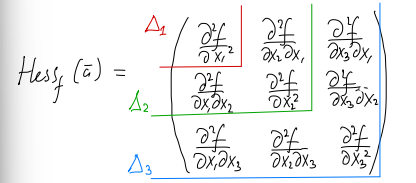
\includegraphics[scale=1.2]{12025-04-30.png}
    \end{center}
\end{parag}


\begin{parag}{Min et Max d'une fonction conitnue sur un ensemble compact}
   \begin{subparag}{Rappel}
       \begin{theoreme}
       Une fonction \important{continue} sur un sous-ensemble \important{compact} $D \subset \mathbb{R}^n$. atteint son min et sont maximum . Formellement:
       \begin{align*} \exists \overline{c_1} \in D: f\left(\overline{c_1}\right) = \text{min}_{\overline{x}\in D}f\left(\overline{x}\right) \\
           \exists \overline{c_2} \in D : f\left(\overline{c_2}\right) = \text{max}_{\overline{x}\in D} f\left(\overline{x}\right)
       \end{align*}
       \end{theoreme}
       
       Pour trouver $\overline{c_1}$ et $\overline{c_2}$ il faut:
       \begin{enumerate}
           \item Trouver les points critiques $\{\overline{c_1}\}$ de $f$ sur $D$ (avec la frontière)
           \item Trouver les points $\{\overline{d_j}\}$ de min, max de $f\left( \nabla D\right)$ calculer les valeurs de $f\left(\overline{d_j}\right)$
           \item Choisir le min et le max de $\{f\left(\overline{c_i}\right), f\left(\overline{d_j}\right)\}$
       \end{enumerate}
   \end{subparag} 
   \begin{subparag}{Exemple}
       $f\left(x, y\right) = 6x^2 + 2x^2y - 3y^2 + 2y + 1$ Trouver le min et le max absolus (global) de $f$ sur le carré $E = \{-2 \leq x, y \leq 2\}$.\\
       La première étape et sur l'ensemble $E = \{-2 < x, y < 2\}$ \\
       On calcule les dérivée partielles:
       \begin{align*} \frac{\partial f}{\partial x} = -12x + 4xy = 4x\left(3-y\right) = 0 \end{align*}
       Qui arrive lorsque $x = 0$ ou $y = 3$ qui n'est pas dans notre ensemble, et donc: $-6y + 2 = 0 \implies y = \frac{1}{3}$, $\left(0, \frac{1}{3}\right) \in E$ .\\
       De l'autre côté:
       \begin{align*} \frac{\partial f}{\partial y} = 2x^2 - 6y + 2 \end{align*}
       En calculant les dérivée partielle seconde:
       \begin{align*} \frac{\partial^2 f }{\partial x^2} = -12 + 4y\\
       \frac{\partial^2 f}{\partial y^2} = -6\\
        \frac{\partial^2 f}{\partial x \partial y} = 4x 
   \end{align*}
   Ce qui implique lorsqu'on calcule la Hessienne:
   \begin{align*} Hess_f\left(0, \frac{1}{3}\right) = \begin{pmatrix} -12 + \frac{4}{3} & 0 \\ 0 & -6 \end{pmatrix} \left(0, \frac{1}{3}\right) \end{align*}
   Et on voit que le déterminant de cette matrice est plus grande que $0$ et que tout les valeurs propres sont négative ($\det > 0$ et $\lambda_i < 0$ nous donne que tout les valeurs propres sont négative (les deux seulement). Ce qui nous donne un maximum locale sur $E$ avec la frontière en $\left(0, \frac{1}{3}\right)$.
       
   \end{subparag}
   \begin{subparag}{Min et Max de $f$ sur la frontière de E}
       Maintenant on cherche le miniment et maximum sur la frontière directement tel que:
       \begin{align*} f\left(x, y\right)_{x = \pm 2} = -24 + 8y - 3y^2 + 2y + 1 \\
       = -3y'2 + 10 y - 23 = g\left(y\right)\end{align*}
       \begin{align*} g'\left(y\right) = -6y + 10 \implies y \frac{5}{3} \end{align*}
       Ce qui nous donne comme élément de l'ensemble $\left(\pm 2, \frac{5}{3}\right)$.\\
       Du côté du $y$:
       \begin{align*} f\left(x, y\right)_{y = 2} = -6x^2 + 4x^2 -12 + 4 + 1 = -2x^2 - 7 = h_1\left(x\right) \implies \left(0, 2\right) \text{ est un max local} \end{align*}
       Avec $h_1'\left(x\right) = -4x, h_1''\left(x\right) = -4 < 0$.\\
       \begin{align*} f\left(x, y\right)_{y = -2} = -6x^2 - 4x^2 -12 -4 + 1 = -10x^2 - 15 = h_2\left(x\right) \implies \left(0, -2\right) \text{ este un max local} \end{align*}
       Avec $h_2'\left(x\right) = -20x$ et $h_2''\left(x\right) = -20 < 0$.\\
       On regarde finalement les coins:
        \begin{align*} f\left(\pm 2, 2\right) = -15\\
        f\left(\pm 2, -2 \right) = -55\end{align*}
        On cherche donc sur toute les valeurs qu'on a trouvées le min et le max qui nous donne $\frac{4}{3}$ pour le max global sur $E$ et $-55$ le minimum global sur $E$. avec:
        \begin{align*} f\left(0, \frac{1}{3}\right) = \frac{4}{3}\\
        f\left(\pm 2, -2\right) = -55 \end{align*}

       
   \end{subparag}
\end{parag}


\subsection{Théorème des fonctions implicites}
\begin{parag}{Question}
    Fonction implicite: Une dépendance $f = f\left(\overline{x}\right)$ qui est définie par une équation.\\
   La question posée est, est ce que l'équation $F\left(x, y\right) = 0$ définit une fonction $y = y\left(x\right)$? 
   \begin{subparag}{Exemple 1}
        Soit $F\left(x, y\right) = x + 3y = 0$\\
        On voit ici que a fonction $y = f\left(x\right)$ et donnée par: $y = - \frac{1}{3}x$ et on voit que cela est définit partout.
   \end{subparag}
   \begin{subparag}{Exemple 2}
       Soit la fonction $F\left(x, y\right) = x^2 + y^2 - 1 = 0$. Et soit $\left(a, b\right) \in$ le cercle, alors $a^2 + b^2 + 1 = $
       Si $b > 0 \implies y = \sqrt{1 - x^2}$ au voisinage de $\left(a, b\right)b > 0$\\
       Si $b < 0 0> y = -\sqrt{1-x^2}$ au voisinage de $\left(a, b\right)$:  $b < 0$.
       Si $b = 0$ on a deux solution pour chaque $x$ dans le voisinage $\left(\pm 1, 0\right)$
   \end{subparag}
    
\end{parag}


\begin{parag}{Surface}
    \begin{definition}
        Une surface (\important{ligne}) de niveau d'une fonction $F\left(x, y, z\right)$ ou ($F\left(x, y\right)$) est la surface (ligne) définie par l'équation
        \begin{align*} F\left(x, y, z\right) = C , \; \; C \in \mathbb{R}\end{align*}

    \end{definition}
    
    \begin{subparag}{Exemple 3}
        soit la fonction $F\left(x, y\right) = 2-ye^x + xe^y$ on cherche $y = f\left(x\right)$ autour d'une point donné $\left(0, 1\right)$?\\
        \begin{center}
            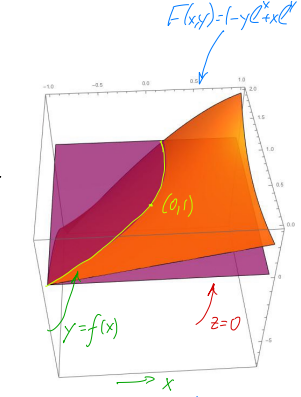
\includegraphics[scale=0.8]{22025-04-30.png}
        \end{center}
        Soit $\left(x, y\right) = \left(0, 1\right)$. On vérifie que $F\left(x, y\right) = 0$ définit autour de $\left(0, 1\right)$ une fonction $y = f\left(x\right)$ telle que $F\left(x, f\left(x\right)\right)= 0$ au voisinage de $x = 0$ et trouver  $f'\left(0\right)$.\\
        On trouve d'abord:
        \begin{align*} \frac{\partial F}{\partial y}= -e^x xe^y \text{ en (0, 1) } = -1 \neq 0 \end{align*}
        Ce qui implique que le TFI est appliquable.\\
        Il existe alors une fonction $f\left(x\right)$ tel que $y = f\left(x\right)$au voisinage de $\left(0, 1\right)$: $F\left(x, f\left(x\right)\right) = 0$. et
        \begin{align*} f'\left(x\right) = -\frac{\frac{\partial F}{\partial x}\left(x, y\right)}{\frac{\partial F}{\partial y}\left(x, y\right)} =- \frac{ye^x + e^y}{-e^x + xe^y}_{\left(0, 1\right)} = -\frac{-1 + e}{-1} = -1 + e = f'\left(0\right) \end{align*}
        On a donc pour l'equation de la tangente au point $\left(0, 1\right)$ à la courbe $y = f\left(x\right)$.
        \begin{align*} y - 1 = \left(-1 + e\right)\left(x - 0\right)\\
        y = 1 + \left(e-1\right)x\end{align*}
        
        
    \end{subparag}
\end{parag}
\begin{parag}{Théorème des fonctions implicites}
    \begin{theoreme}
    $F: E \to \mathbb{R}$ une fonction de classe $C^1$ au voisinage de $\overline{a} = \left(a_1, \ldots, a_n\right) \in E$ telle que:
   \begin{align*} 
       F\left(\overline{a}\right) &= 0\\
       \frac{\partial F}{\partial x_n}\left(\overline{a}\right) &\neq 0
   \end{align*}
   Alors il existe un voisinage $B\left( \overline{a}', \delta\right)$ de $\overline{a}' = \left(a_1, a_2, \ldots, a_{n-1}\right)\in \mathbb{R}^{n-1}$ et une fonction $f : B\left(\overline{a}', \delta\right) \to \mathbb{R}$ telle que\\
   \begin{enumerate}
       \item $a_n = f\left(a_1, \ldots a_{n-1}\right)$
       \item $F\left(x_1, x_2, \ldots, x_{n-1}, f\left(x_1, \ldots, x_{n-1}\right)\right) = 0 $ et cela $\forall \left(x_1, x_2, \ldots, x_{n-1}\right) \in B\left( \overline{a}', \delta\right)$.
   \end{enumerate}
   
    \end{theoreme}
    De plus, $f$ est de classe $C^1$ dans un voisinage de $\overline{a}'$ et on a
    \begin{align*} \frac{\partial f}{\partial d_p} \left(x_1, x_2, \ldots, x_{n-1}\right) = - \frac{\frac{\partial F}{\partial x_p}\left(x_1, \ldots, x_{n-1}, f\left(x_1, \ldots, x_{n-1}\right)\right)}{\frac{\partial F}{\partial x_n}\left(x_1, \ldots, x_{n-1}, f\left(x_1, \ldots, x_{n-1}\right)\right)} \; \; \forall p \in \{1, \ldots, n-1\} \end{align*}

\end{parag}
\begin{parag}{Cas particulier du TFI: deux variables}
    Soit $F\left(x, y\right): E \to \mathbb{R}$ de classe $C^1$ telle que $F\left(a,b\right) = 0$ et $\frac{\partial F}{\partial y}\left(a, b\right) \neq 0$.\\
    Alors l'équation $F\left(x, y\right) = 0$ définit localement autour de $\left(a, b\right)$ une fonction $y = f\left(x\right) $ telle que:
    \begin{enumerate}
        \item $f\left(a\right) = b$
        \item $F\left(x_1, f\left(x\right)\right) = 0$
        \item $f'\left(x\right) = - \frac{\frac{\partial F}{\partial x}\left(x, f\left(x\right)\right)}{\frac{\partial F}{\partial y}\left(x, f\left(x\right)\right)}$
    \end{enumerate}
    Cela veut dire que l'on peut calculer $f'\left(a\right)$ sans savoir la formule explicite pour $f\left(x\right)$.
    
\end{parag}

\begin{parag}{Cas particulier du TFI: trois variables}
    Soit $F\left(x, y, z\right): E \to \mathbb{R}$ de classe $C^{1}$ tel que $F\left(a,b, c\right) = 0$ et $\frac{\partial F}{\partial z}\left(a, b, c\right) \neq 0$.\\
    Alors il existe localement une fonction $z = f\left(x, y\right)$ telle que 
    \begin{enumerate}
        \item $f\left(a, b\right) = c$
        \item $F\left(x, y, f\left(x, y\right)\right) = 0$ pour tout couple, $\left(x, y\right)$ dans un voisinage de $\left(a, b\right)$
        \item $\frac{\partial f}{\partial x}\left(x, y\right) = - \frac{\frac{\partial F}{\partial x}\left(x, y, f\left(x, y\right)\right)}{\frac{\partial F}{\partial z}\left(x, y, f\left(x, y\right)\right)}$; $\partial $ je ferais après
        
    \end{enumerate}
    
    
\end{parag}

\begin{parag}{Q16}
    L'équation $F\left(x, y\right) = \sin\left(x + y\right)\cos\left(x-y\right) - \frac{1}{2} = 0$. On cherche $g\left(x\right)$.\\
\begin{align*} \frac{\partial F}{\partial x}\left(x, y\right) = \cos\left(x + y\right)\cos\left(x-y\right) - \sin\left(x + y\right)\sin\left(x-y\right) \end{align*}
\begin{align*} \frac{\partial F}{\partial y}\left(x, y\right) = \cos\left(x + y\right)\cos\left(x-y\right) + \sin\left(x+y\right)\sin\left(x-y\right) \end{align*}

Donc si on simplifie:
\begin{align*} \frac{\cos\left(2x\right)}{\cos\left(2y\right)} \end{align*}
    On pose les questions: $\exists x =  h\left(y\right)$ et $\exists y =  g\left(x\right)$ et nous voyons que cela est vrai seulement pour $x = h\left(y\right)$.:\\
Comme dit précédemment on trouve donc la dérivée de la fonction grâce a notre formule:
\begin{align*} h'\left(y\right) = - \frac{\frac{\partial F}{\partial y}}{\frac{\partial F}{\partial x}}_{\left(\frac{\pi}{2}, \frac{\pi}{4}\right)} = -\frac{0}{-1}\end{align*}
On obtient logiquement pour la pente de la tangent $x =  h\left(y\right)$ en $\left(\frac{\pi}{2}, \frac{\pi}{4}\right)$ est $0$.

\end{parag}



